\mathversion{bold}
\chapter{Sequence Analysis of \s{} factors}
\mathversion{normal}

\section{Introduction}

There are a plethora of \s{} factor sequences submitted to
databases in recent years. Yet, a detailed analysis of primary
sequences of the \s{} factors, particularly, comparative genomics
data elucidating the evolution of \s{} factors is yet to come.
This Chapter is the results of one such attempt.

In this Chapter the results of a detailed sequence comparison of
the primary \s{} factors from the viewpoint of cold-adaptation,
followed by the sequence comparison of \e{rpoS} is discussed. The
discussion on \e{rpoS} is primarily focused on  information that
could be derived from the sequence comparison on the regulation of
\e{rpoS} in Lz4W.

\section{Results}

\mathversion{bold}
\subsection{Sequence comparison of primary \s{} factors}
\mathversion{normal}

Sequences of the primary \s{} factors  were collected from
SwissProt database. There were 44 unique full-length sequences
present in this database. All these sequences with their length
and predicted molecular weight are listed in
Table~\ref{rpod_table}. The collection contained two known
cold-adapted bacteria, the deep-sea barophilic \e{Shewanella
violacea} and psychrotroph \e{Listeria monocytogenes}. A multiple
alignment of these sequences with two sequences of \e{Thermus
aquaticus} and \e{Thermus thermophilus} and Lz4W RpoD (\Lzsiga{})
is shown in Figure~\ref{rpod_align}. It was evident from the
alignment that the cloned fragment of \lzsiga{} contained a part
of non-conserved region between regions 1.2 to 2. The cloned
region also contained the rest of the C-terminal end of the RpoD.
A comparison the sequences with important functions is discussed
below. For all discussion in this Chapter, sequence number will be
referred in terms of \bact{Ec} RpoD.

\begin{table}
\begin{minipage}[c]{\textwidth}
\linespread{1}\normalsize \renewcommand{\arraystretch}{1.3}
\renewcommand{\footnoterule}{}
\caption[Primary \s{} factors in SwissProt database]{Primary \s{}
factors in SwissProt database. Only full-length sequences were
considered. Two sequences of \e{Thermus aquaticus} and \e{Thermus
thermophilus} were collected from GeneBank and the accession
numbers are shown with prefix ``gb:''.} \label{rpod_table}
\begin{narrow}{-1in}{-1in}
\centering
\begin{small}
\begin{tabular}{@{}llllp{.7in}@{}}\toprule
\textbf{Species} & \textbf{Key} & \textbf{Accession} &
\textbf{Length (aa)} & \textbf{Molecular Weight (Da)}\\\midrule
{\it Agrobacterium tumefaciens} & Atumefaciens &     P33452 &        684 &      77399 \\

{\it Anabaena} sp.  &   Anabaena &     P26683 &        390 &      45641 \\

{\it Bacillus halodurans} & Bhalodurans &     O66381 &        372 &      42740 \\

{\it Bacillus subtilis} &  Bsubtilis &     P06224 &        371 &      42957 \\

{\it Borrelia burgdorferi } & Bburgdorferi &     P52323 &        631 &      73642 \\

{\it Buchnera aphidicola } & Baphidicola &     P32001 &        617 &      71469 \\

{\it Caulobacter crescentus} & Ccrescentus &     P52324 &        652 &      72675 \\

{\it Chlamydia muridarum} & Cmuridarum &     P56835 &        571 &      66196 \\

{\it Chlamydia pneumoniae } & Cpneumoniae &     Q9Z7F0 &        572 &      66305 \\

{\it Chlamydia trachomatis} & Ctrachomatis &     P18333 &        571 &      66133 \\

{\it Clostridium acetobutylicum} & Cacetobutylicum &     P33656 &        378 &      43260 \\

{\it Enterococcus faecalis} &  Efaecalis &     P52329 &        368 &      41845 \\

{\it Escherichia coli} &      Ecoli &     P00579 &        613 &      70263 \\

{\it Haemophilus influenzae} & Hinfluenzae &     P43766 &        629 &      72084 \\

{\it Helicobacter pylori} &    Hpylori &     P55993 &        671 &      77737 \\

{\it Helicobacter pylori} J99  & HpyloriJ99 &     Q9ZMY3 &        681 &      78763 \\

{\it Lactococcus lactis} (subsp. \e{cremoris}) & Llactiscremoris &     P58290 &        364 &      41579 \\

{\it Lactococcus lactis} (subsp. \e{lactis})  & Llactislactis &     P52330 &        386 &      44079 \\

{\it Leptospira interrogans} & Linterrogans &     P52328 &        377 &      43456 \\

{\it Listeria innocua} &   Linnocua &     Q92BQ6 &        374 &      42446 \\

{\it Listeria monocytogenes} & Lmonocytogenes &     P52331 &        374 &      42419 \\

{\it Microcystis aeruginosa} & Maeruginosa &     P52322 &        416 &      48871 \\

{\it Mycobacterium bovis} &     Mbovis &     Q60162 &        528 &      57800 \\

{\it Mycoplasma genitalium} & Mgenitalium &     P47491 &        497 &      57661 \\

{\it Mycoplasma pneumoniae} & Mpneumoniae &     P78022 &        499 &      57796 \\

{\it Myxococcus xanthus} &   Mxanthus &     P17531 &        708 &      80398 \\

{\it Neisseria gonorrhoeae} & Ngonorrhoeae &     P52325 &        642 &      73679 \\

{\it Pseudomonas aeruginosa} & Paeruginosa &     P26480 &        617 &      69643 \\

{\it Pseudomonas fluorescens} & Pfluorescens &     P52326 &        615 &      69436 \\

{\it Pseudomonas putida} &    Pputida &     P52327 &        614 &      69725 \\

{\it Rhizobium meliloti}  &  Rmeliloti &     Q59753 &        684 &      77173 \\

{\it Rhodobacter capsulatus} & Rcapsulataus &     P46400 &        674 &      75958 \\

{\it Rickettsia prowazekii} & Rprowazekii &     P33451 & 635 &
73080 \\\bottomrule


%\end{minipage}
\end{tabular}
\end{small}
\end{narrow}
\end{minipage}
\linespread{1.1}\normalsize
\end{table}
\begin{table}

\begin{minipage}[c]{\textwidth}
\linespread{1}\normalsize
\renewcommand{\arraystretch}{1.3}
\renewcommand{\footnoterule}{}
\centering {\sffamily\footnotesize\textbf{TABLE~\ref{rpod_table}}\
\ \ \e{Continued.}}\vspace{1em}
\begin{narrow}{-1in}{-1in}
\centering
\begin{small}
\begin{tabular}{@{}llllp{.7in}@{}}\toprule
\textbf{Species} & \textbf{Key} & \textbf{Accession} &
\textbf{Length (aa)} & \textbf{Molecular Weight (Da)}\\\midrule
{\it Salmonella typhimurium} & Styphimurium &     P07336 &        615 &      70530 \\

{\it Shewanella violacea} &  Sviolacea &     O24744 &        614 &      70030 \\

{\it Staphylococcus aureus} &    Saureus &     P26766 &        368 &      42170 \\

{\it Staphylococcus aureus (N315)} & SaureusN315 &     Q99TT5 &        368 &      42156 \\

{\it Streptococcus mutans} &    Smutans &     O33662 &        371 &      42547 \\

{\it Streptococcus pneumoniae} & Spneumoniae &     O08388 &        369 &      42030 \\

{\it Streptomyces aureofaciens} & Saureofaciens &     P27785 &        317 &      35616 \\

{\it Synechococcus} sp. (PCC 7942) & Synechococcus &     P38023 &        384 &      44123 \\

{\it Thermotoga maritima} &  Tmaritima &     P77994 &        399 &      46534 \\

{\it Thermus aquaticus} & Taquaticus & gb:AAG36964 &        438 &      49846 \\

{\it Thermus thermophilus} & Tthermophilus & gb:BAA74758 &        423 &      48494 \\

{\it Treponema pallidum} &  Tpallidum &     O83506 &        611 &      70902 \\

{\it Xylella fastidiosa} & Xfastidiosa &     Q9PDM9 &        618 &
69907 \\\bottomrule
\end{tabular}
\end{small}
\end{narrow}
\end{minipage}
\linespread{1.1}\normalsize
\end{table}
\FloatBarrier


\subsubsection{Core-binding region of RpoD}

As discussed in the Section~\ref{chap1:core_binding}, region 2.2
of \s{} factor, makes extensive contact with the $\betaup'$
subunit. Comparison of these regions showed that, the first three
residues are part of coil and rest is an $\alphaup$ helix. All the
amino acids in this region of \lzsiga{} are identical with the
corresponding residues of other pseudomonads and \bact{Ec}
(Figure~\ref{rpod_align}).

\subsubsection{$-$10 binding and promoter melting}

In Section~\ref{chap1:melting}, it was discussed that the basic
and the aromatic residues in the region 2.3 help in the nucleation
of the strand separation during open complex formation. Comparison
of this region between the cold-adapted species and the
thermophiles revealed that in \e{Thermus} species absolutely
conserved G426 has been replaced by a R residue. All the
differences other than this residues were conserved replacement.
In fact the $\alphaup$ helical portion of this region is
absolutely conserved in all species, particularly, Y430, W433, and
K418 (cyan $\ast$ in Figure~\ref{rpod_align}), which have been
implicated in stacking A($-$11) of the promoter and stabilizing
the separated strands. K414, which is also believed to stabilize
the separated strands, on the other hand is sometimes replaced by
R in many species.

\begin{sidewaysfigure}[tbp]
\centering
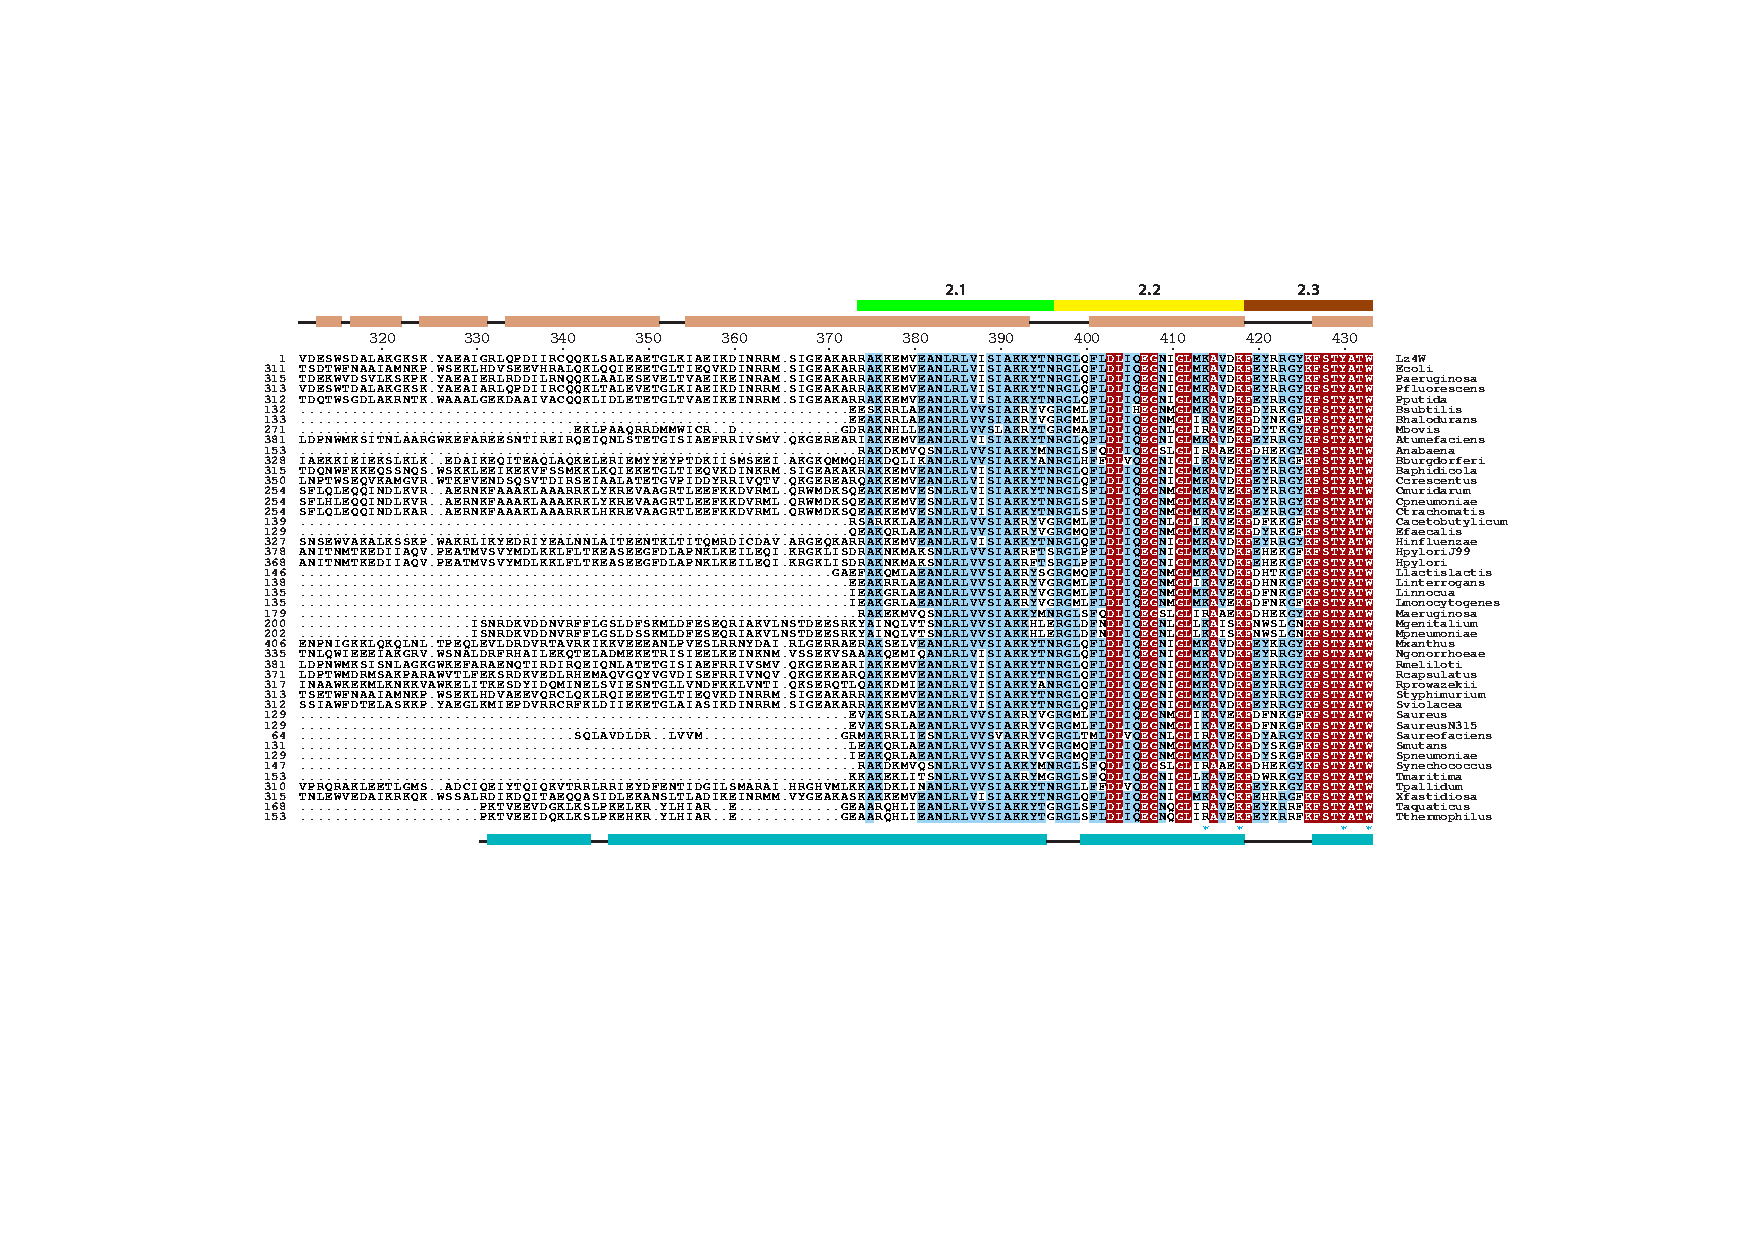
\includegraphics{figures/chap4_rpod_align_1}
\caption[Multiple sequence alignment of primary \s{}
factors]{Multiple sequence alignment of primary \s{} factors. All
full-length primary \s{} factors from SwissProt database (see
Table~\ref{rpod_table} for the accession numbers and the name
keys) were aligned using CLUSTALW~\citep{Higgins1996}. The colored
bars on the topmost position showed regions of \s{}, colored as in
Figure~\ref{chap1:sigma}. The tan bars and lines on top indicate
$\alphaup$ helices and coils as in \bact{Ec} \s\smallsu{70}
fragment crystal structure~\citep[][PDB coordinate
1SIG]{Malhotra1996}. The blue bars, the lines, and the dotted
lines below represent the $\alphaup$ helices, coils, and
disordered region observed in \e{T. thermophilus} \s\smallsu{A}
crystal structure~\citep[][PDB coordinate 1IW7]{Vassy2002}. The
ruler numbering indicates \bact{Ec} residue number. The numbering
for Lz4W RpoD corresponds to the internal residue position, for
which the sequence information obtained in the present study. The
N-terminal sequence information is lacking. Important residues are
marked with ``$\ast$'' and colored according to function; promoter
melting, cyan; $-$10 recognition, red; extended $-$10 recognition,
green; $-$35 recognition, blue.} \label{rpod_align}
\end{sidewaysfigure}
\begin{sidewaysfigure}[tbp]
\centering
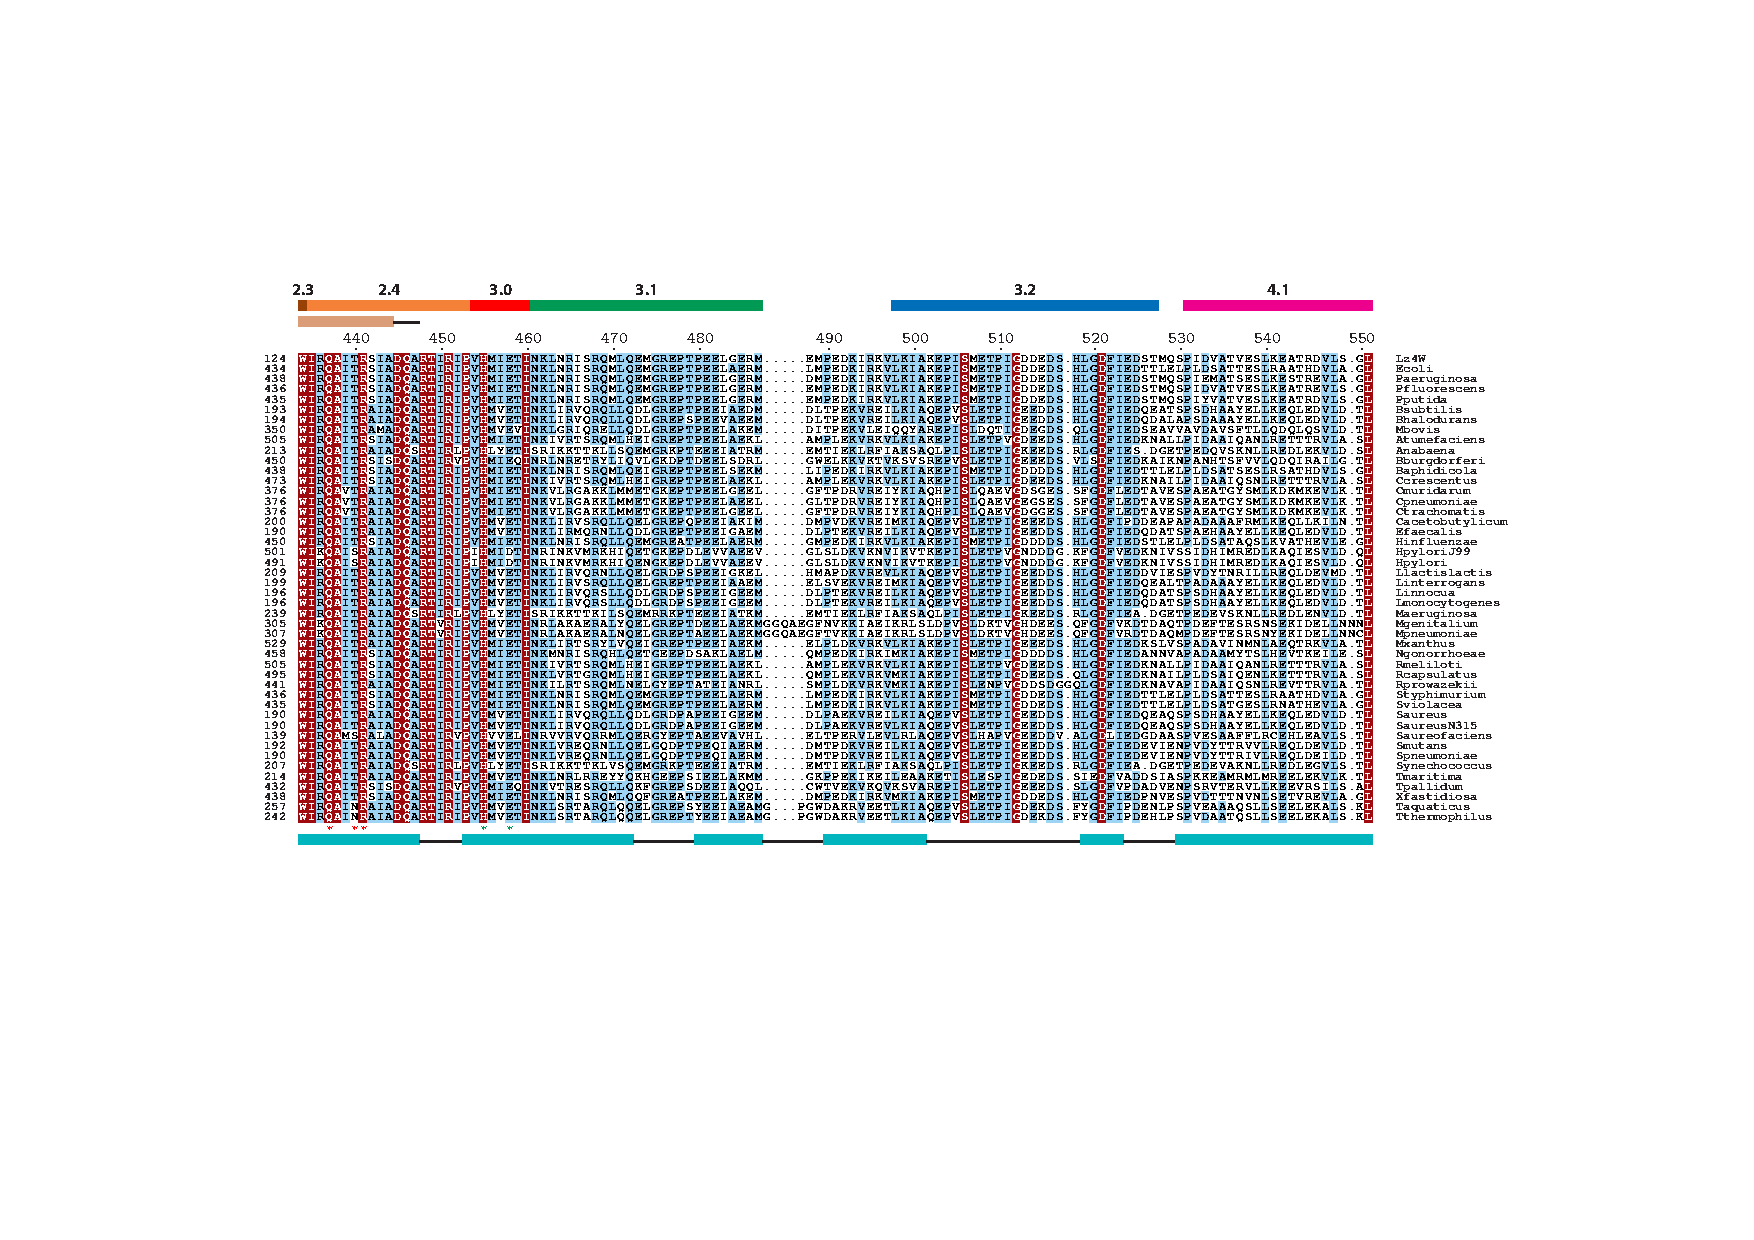
\includegraphics{figures/chap4_rpod_align_2}
{\footnotesize\bfseries\sffamily
FIGURE~\ref{rpod_align}}~{\footnotesize\sffamily\itshape\
Continued.}
\end{sidewaysfigure}
\begin{sidewaysfigure}[tbp]
\centering
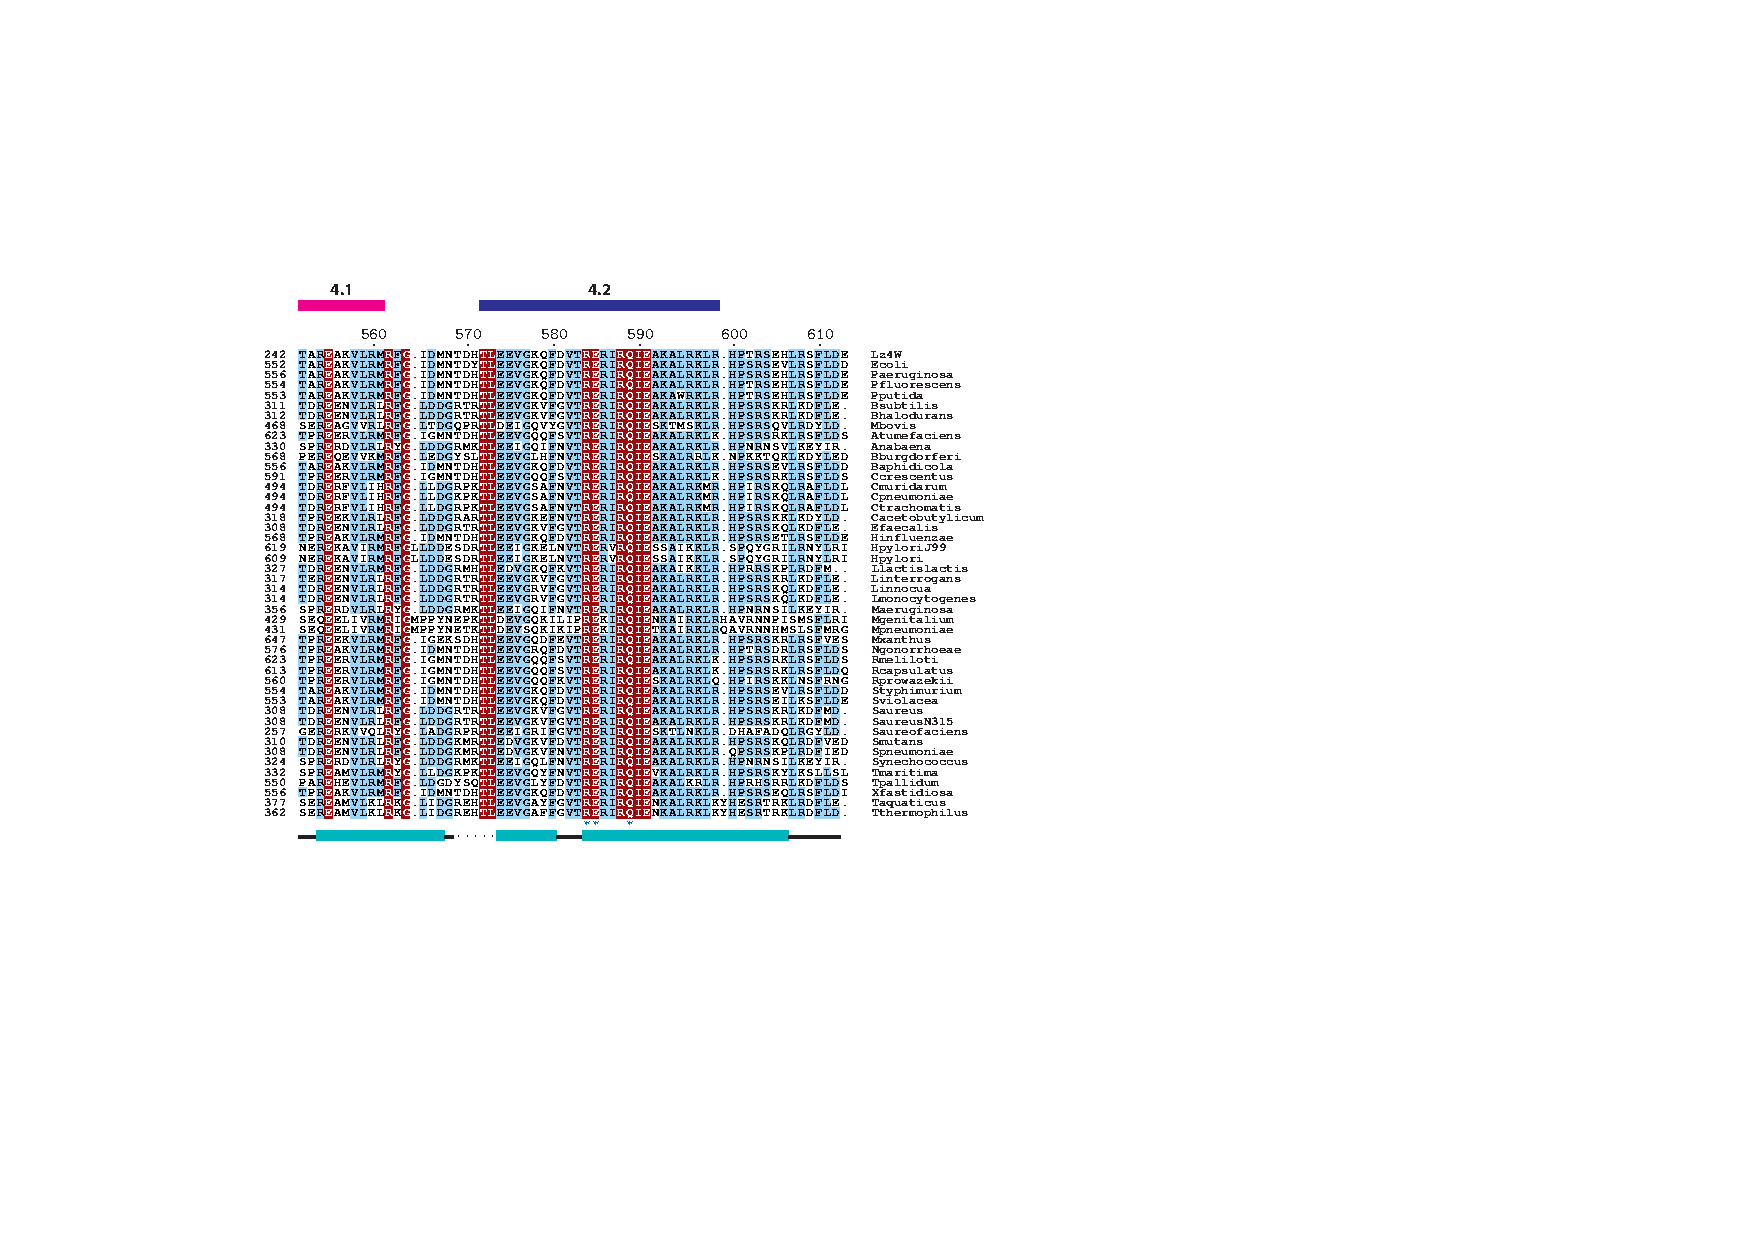
\includegraphics{figures/chap4_rpod_align_3}
{\footnotesize\bfseries\sffamily
FIGURE~\ref{rpod_align}}~{\footnotesize\sffamily\itshape\
Continued.}
\end{sidewaysfigure}

Q437 and T440, which have been shown to contact T($-$12) and R441,
which has been shown to contact $-$13 nucleotide of the promoter
are part of the same $\alphaup$ helix and are also either
conserved, or replaced by similar amino acids in all species (red
$\ast$ in Figure~\ref{rpod_align}).

H455 and E458 have been shown to contact extended $-$10 of the
promoter. Among these H455 is absolutely conserved, whereas E458
has been replaced by a conservative charged residue D in
\e{Helicobacter} (green $\ast$ in Figure~\ref{rpod_align}).

\subsubsection{$-$35 contact sites}

R584, E585 and Q589 of the region 4.2 are the major contact point
of $-$35 site of the promoters. These residues are absolutely
conserved in all bacterial species (blue $\ast$ in
Figure~\ref{rpod_align}).


\subsection{RpoS sequence comparison}

Till date there are 27 unique sequences (full-length) available
for \sigs{} in SwissProt/TrEMBL database. All these sequences with
their predicted molecular weights and lengths are listed in
Table~\ref{chap4:rpos_table}. Except three species from $\betaup$
Proteobacteria and \e{Aquifex}, all other sequences are from
$\gammaup$ Proteobacteria. A multiple alignment of these sequences
with the Lz4W sequence is shown in Figure~\ref{rpos_align}. As
evident from the alignment the reported \e{rpoS}-like sequences
from $\betaup$ Proteobacteria and \e{Aquifex} are quite different
from RpoS sequences from $\gammaup$ Proteobacteria.

\begin{table}
\begin{minipage}[c]{\textwidth}
\renewcommand{\footnoterule}{}
\caption[Known \emph{rpoS} sequences]{\emph{rpoS} sequences in
SwissProt and TrEMBL databases till September,
2002\protect\footnote{Only full-length sequences are shown.
Truncated or incomplete sequences are not considered.}.}
\label{chap4:rpos_table}
\begin{narrow}{-1in}{-1in}
\centering
\begin{small}
\begin{tabular}{@{}llp{.8in}p{.8in}p{.7in}@{}}\toprule
\textbf{Species} & \textbf{Key} & \textbf{Swiss\-Prot/\-Tr\-EMBLE
accession} & \textbf{Length (amino acids)} & \textbf{Molecular
Weight (Da)}\\\midrule\addlinespace
{\it Aquifex aeolicus} & Aaeolicus & O67437 & 310 & 35777 \\

{\it Azotobacter vinelandii} & Avinelandii & Q93AG3 & 334 & 38305 \\

{\it Burkholderia cepacia}  & Bcepacia & Q8RKM7 & 362 & 41056 \\

{\it Enterobacter cloacae} & Ecloacae & O08372 & 346 & 39575 \\

{\it Erwinia carotovora} & Ecarotovora & P77860 & 330 & 38014 \\

{\it Erwinia chrysanthemi} & Echrysanthemi & Q93KA2 & 332 & 38389 \\

{\it Escherichia coli} & Ecoli & P13445 & 330 & 37971 \\

{\it Escherichia coli} O157:H7 & Ecoli\_O157 & Q8XEE1 & 330 & 38058 \\

{\it Kluyvera citrophila } & Kcitrophila & O32708 & 345 & 39534 \\

{\it Legionella pneumophila} & Lpneumophila & Q9S4T1 & 341 & 39449 \\

{\it Pseudomonas aeruginosa} & Paeruginosa & P45684 & 334 & 38235 \\

{\it Pseudomonas fluorescens} & Pfluorescens & Q59664 & 335 & 38243 \\

{\it Pseudomonas putida} KT2440 & Pputida\_KT2440  & P77927 & 335 & 38183 \\

{\it Pseudomonas putida} WCS358 & Pputida\_WCS358  & Q9WWV5 & 335 & 38198 \\

{\it Pseudomonas syringae} pv. syringae & Psyringae\_S & Q9RBQ6 & 335 & 38193 \\

{\it Pseudomonas syringae} pv. tomato & Psyringae\_T & O69079 & 335 & 38128 \\

{\it Pseudomonas tolaasii} & Ptolaasii & O33503 & 336 & 38482 \\

{\it Ralstonia solanacearum } & Rsolanacearum & Q8Y037 & 377 & 41830 \\

{\it Rhodocyclus gelatinosus } & Rgelatinosa & Q9JP89 & 322 & 36104 \\

{\it Salmonella enterica} & Senterica & P37400 & 330 & 37932 \\

{\it Serratia entomophila} & Sentomophila & Q59904 & 332 & 38288 \\

{\it Shigella flexneri} & Sflexneri & P35540 & 350 & 40113 \\

{\it Vibrio cholerae} & Vcholerae & O51804 & 335 & 38534 \\

{\it Vibrio parahaemolyticus} & Vparahaemolyticus & Q9X6S5 & 321 & 36636 \\

{\it Xenorhabdus nematophilus} & Xnematophilus & Q9RFA4 & 331 & 38183 \\

{\it Yersinia enterocolitica} & Yenterocolitica & P47765 & 331 & 37967 \\

{\it Yersinia pestis} & Ypestis & Q8ZBQ2 & 332 & 38214
\\\addlinespace\bottomrule

\end{tabular}
\end{small}
\end{narrow}
\end{minipage}
\end{table}


\begin{sidewaysfigure}[tbp]
\centering
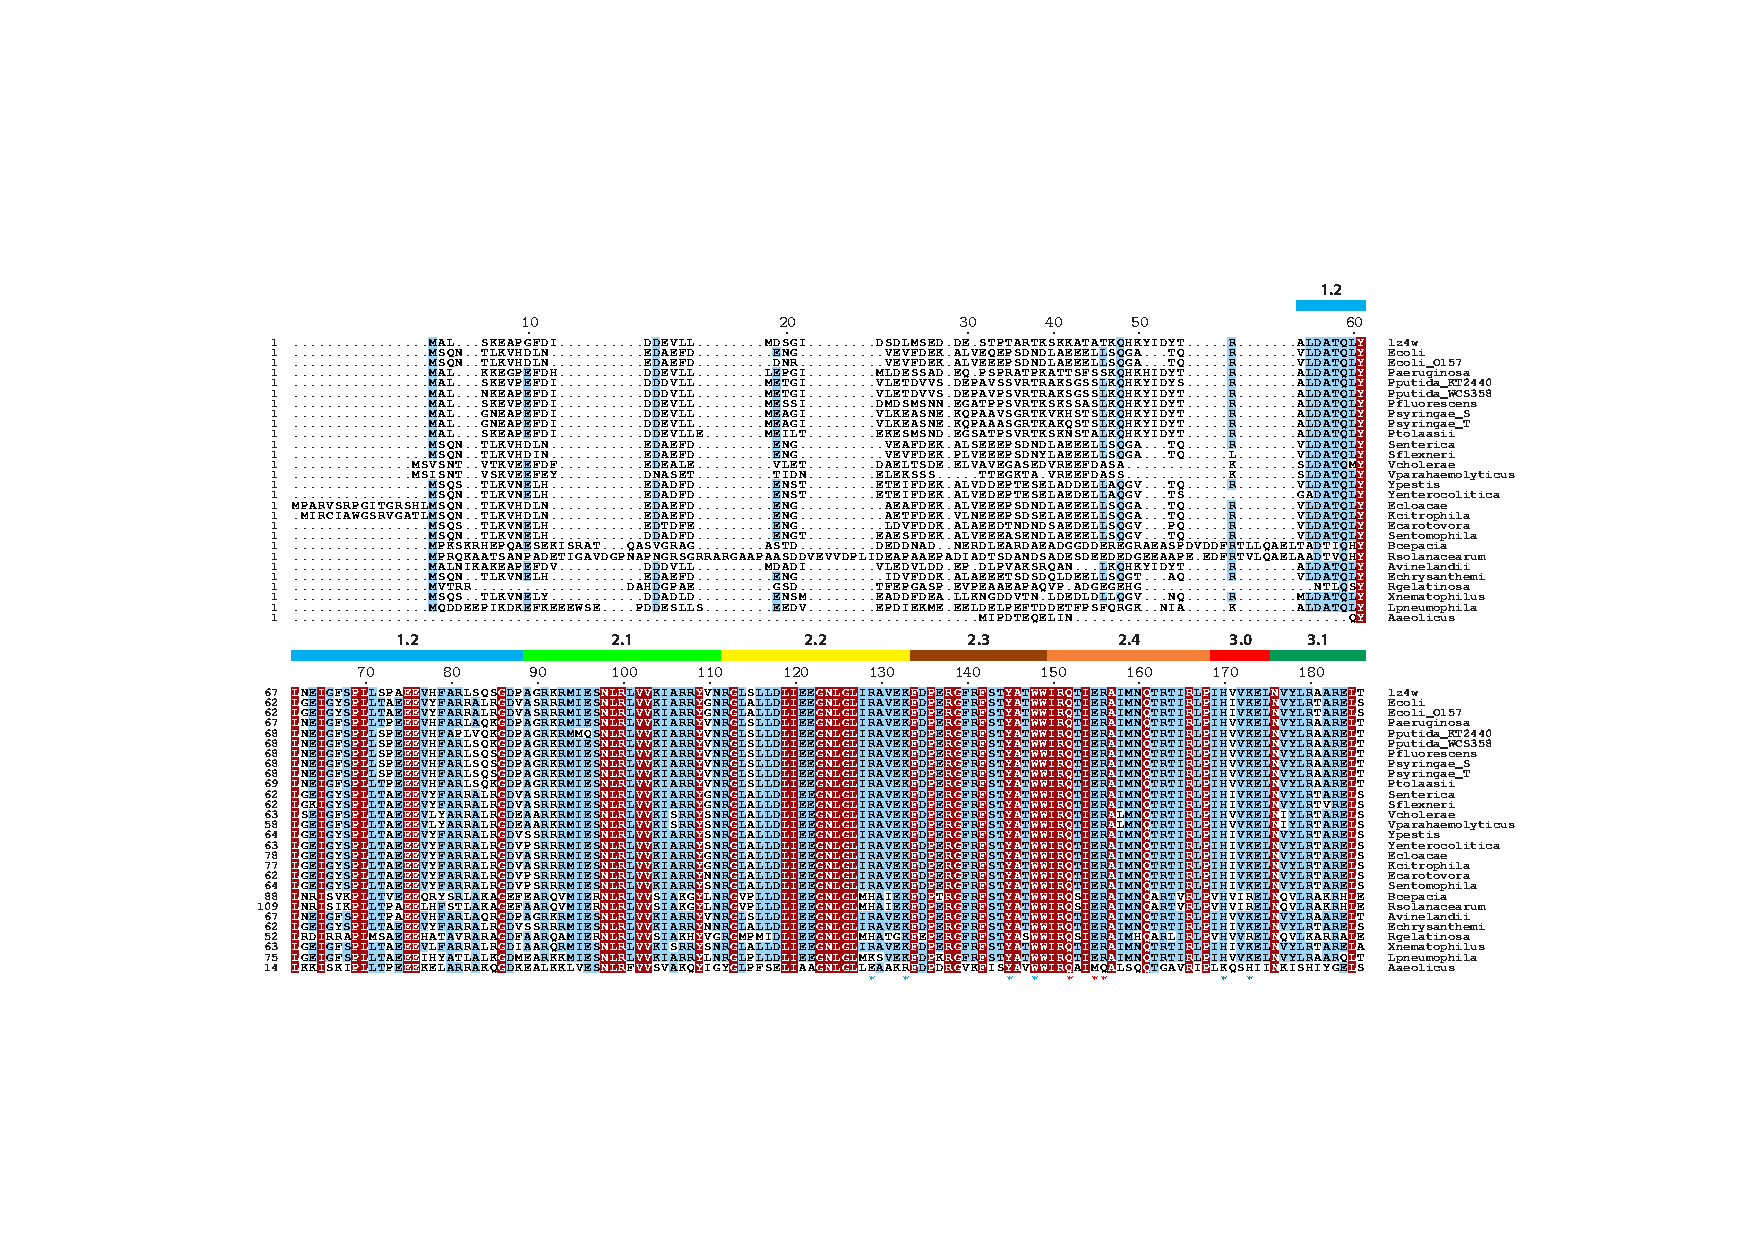
\includegraphics{figures/chap4_rpos_align_1}
\caption[Multiple sequence alignment of RpoS sequences]{Multiple
sequence alignment of RpoS. All full-length RpoS sequences from
SwissProt/TrEMBL database (see Table~\ref{chap4:rpos_table} for
the accession numbers and the name keys) were aligned using
CLUSTALW~\citep{Higgins1996}. The ruler numbering indicates
\bact{Ec} residue number. Important residues by comparison with
the RpoD sequence are marked with ``$\ast$'' and colored according
to function; promoter melting, cyan; $-$10 recognition, red;
extended $-$10 recognition, green; $-$35 recognition, blue. Note
K173 which has been directly shown to contact extended $-$10 and
to bind to RssB, a post-translational stability factor. The amber
mutation in Lz4W RpoS has been replaced by X and marked with black
``$\ast$''.} \label{rpos_align}
\end{sidewaysfigure}
\begin{sidewaysfigure}[tbp]
\centering
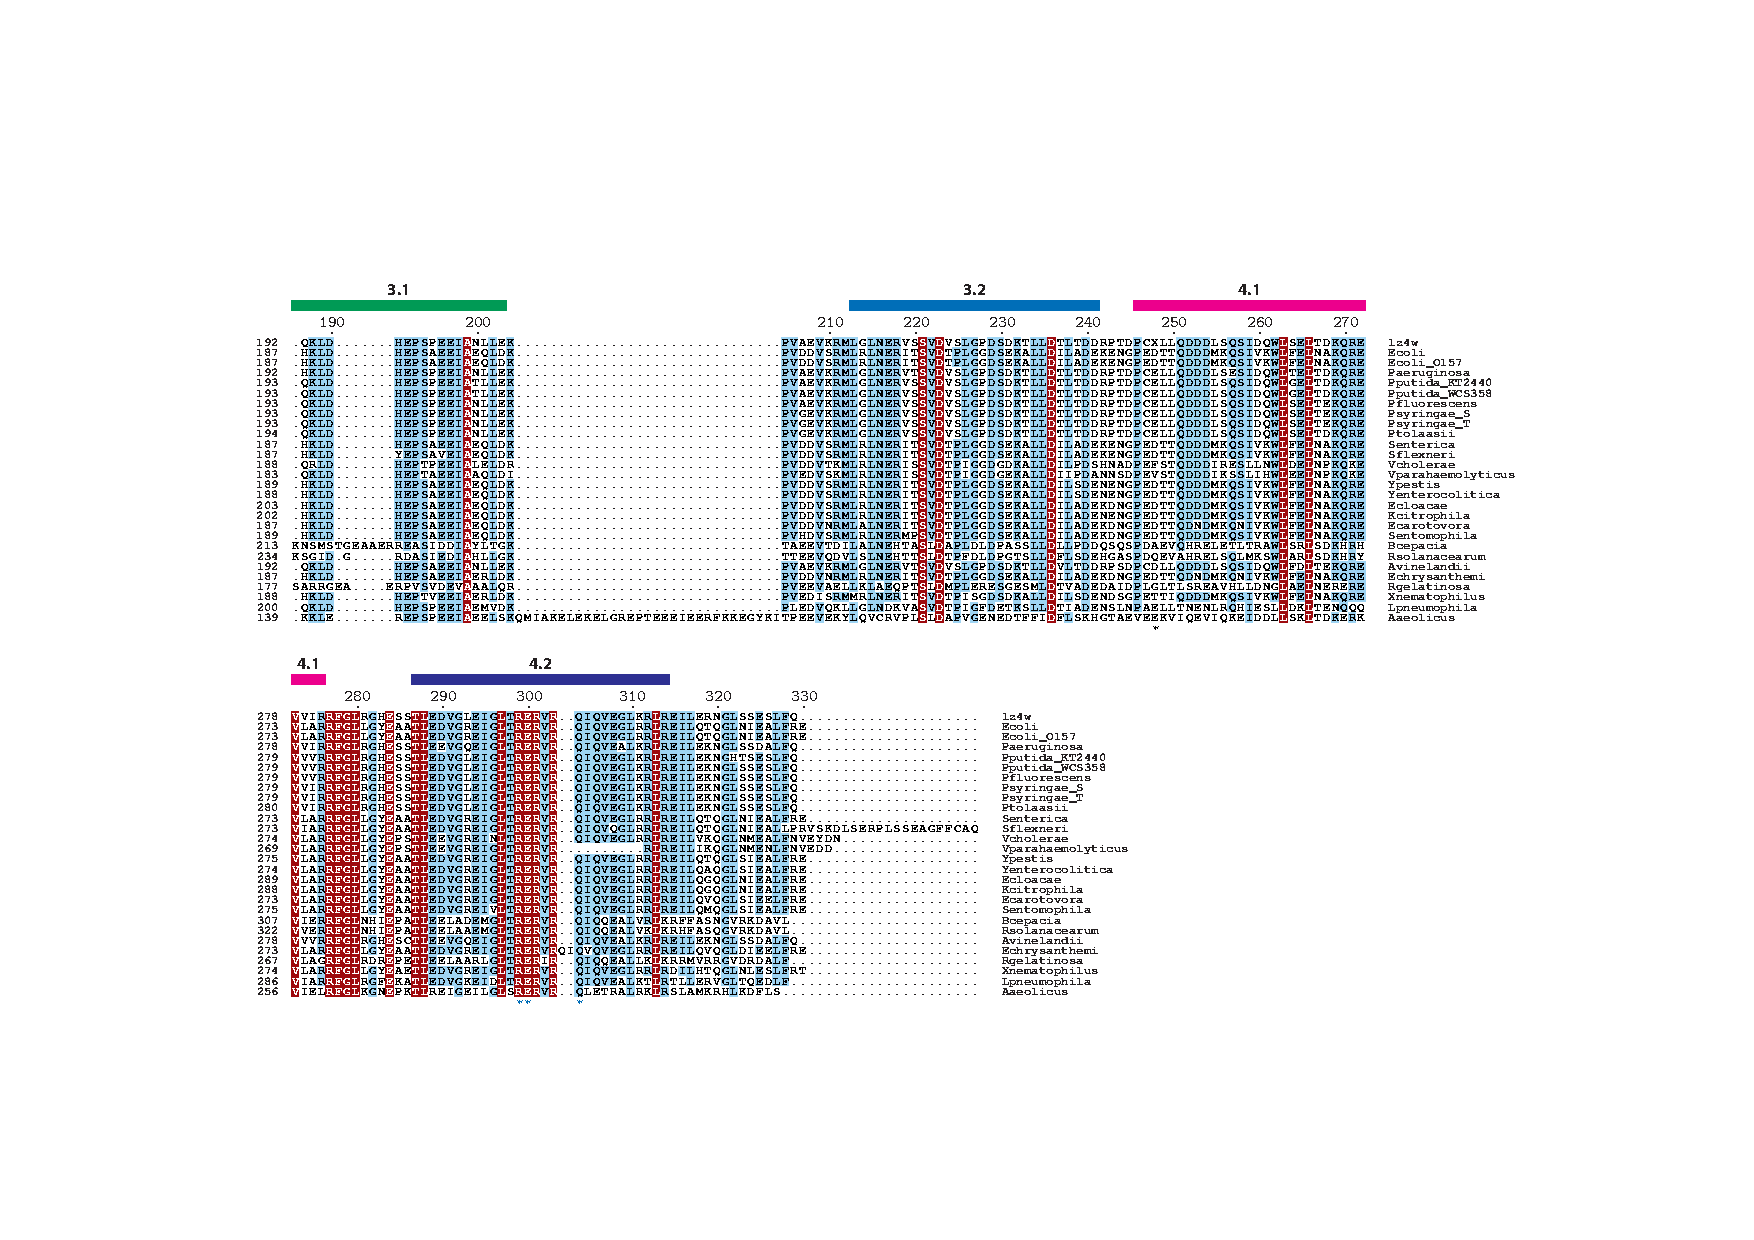
\includegraphics{figures/chap4_rpos_align_2}
{\footnotesize\bfseries\sffamily
FIGURE~\ref{rpos_align}}~{\footnotesize\sffamily\ \ Continued.}
\end{sidewaysfigure}

The first observation from the alignment is that RpoS lacks region
1.1 (Figure~\ref{plotcon}). The similarity index of this region is
below 0.1 (Figure~\ref{plotcon}). This is interesting from the
view that region 1.1 has been implicated in helping in the open
complex formation~\citep[][see also
Section~\ref{region1_1}]{Young2002}.


\begin{figure}[htbp]
\centering
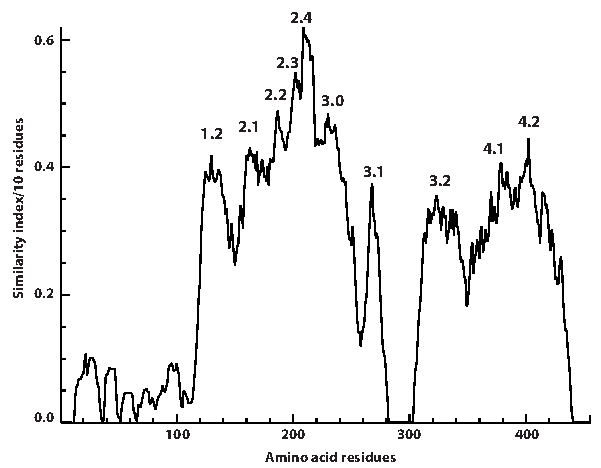
\includegraphics{figures/chap4_plotcon}
\caption[Consensus plot of RpoS sequence alignment]{Consensus plot
of RpoS sequence alignment. Average similarity indices with ten
residues window were calculated from the alignment shown in
Figure~\ref{rpos_align} and plotted in Y-axis against the residue
position in X-axis using PLOTCON program in EMBOSS
package~\citep{Rice2000}.} \label{plotcon}
\end{figure}

It is evident from the alignment that the amber in Lz4W RpoS
(\Lzsigs{}) is at the beginning of region 4.1. If not interrupted
by amber the gene would produce a \sigs{} of 334 amino acids with
molecular weight of \U{38}{KDa} and pI 5.18. The amber at the
codon 253 truncates the protein. The resulting protein would have
a molecular weight of \U{$\sim$28.5}{KDa} with theoretical pI of
5.3.

Although data on functions of individual residues in RpoS sequence
are scanty, a comparison with the RpoD sequence could easily
provide information about the possible important residues in RpoS,
which is discussed below. For all discussion, the residue number
in parenthesis indicates the RpoD residue number.

\subsection{$-$10 binding and promoter melting}

R129(K414), K133(K418), Y145(Y430), W148(W433) of region 2.3 of of
\sigs{} (corresponding residue number of \siga{} are indicated in
parenthesis) are highly con\-served residues (cyan $\ast$ in
Figure~\ref{rpos_align}). Y145 and W148 are conserved in all
species. Outside of pseudomonads and Enterobacteriaceae, R129 is
replaced by a H residue. Q152(Q437) is conserved in all species.
E155(T440) and R156(R441) (red $\ast$ in Figure~\ref{rpos_align})
are conserved in all species except \e{Aquifex}, indicating the
\e{rpoS}-dependent promoters might have a different sequence in
this species. Interestingly T440 of RpoD, which is known to
recognize $-$12 position of the promoter has been replaced by E155
in RpoS.

H170(H455) and K173(E458) are almost fully conserved, indicating
that RpoS might recognize \e{extended $-$10} like RpoD. K173 has
already been shown to contact \seq{C}($-$13)~\citep{Becker2001}.

\subsection{$-$35 binding}

R299(R584), E300(E585), and Q304(Q589) from the region 4.2, which
are involved in the recognition of $-$35 element of the promoter,
are fully conserved as in case of RpoD.

\mathversion{bold}
\subsection{\sigs{} turnover element}
\mathversion{normal}

RssB, a response regulator of a two component pathway has been
shown to recognize K173 of RpoS, and this recognition is essential
for proteolytic degradation of RpoS~\citep[][see also
Section~\ref{chap1_rssb}]{Becker1999}. K173 is conserved in all
$\gammaup$ proteobacteria. All the three species from $\betaup$
proteobacteria (Figure~\ref{rpos_align}), namely \e{R.
solanacearum}, \e{R. gelatinosus}, and \e{B. cepacia} \sigs{} has
R residue at this position. In \e{Aquifex}, K173 has been replaced
by a H residue. Whether this substitution would have any effect on
\sigs{} turnover in these species, is a fact remaining to be
investigated.

\section{\e{rpoS} promoter structure}

An alignment of upstream DNA sequences from Lz4W \e{rpoS}
(\lzsig{}) , \e{P. aeruginosa} \e{rpoS} (\pasig{}) and \e{P.
putida} \e{rpoS} (\ppsig{}) was carried out to find common
\e{cis}-acting elements for transcriptional regulation of the
\e{rpoS}. The alignment immediately revealed the similarity of the
promoters of these genes (Figure~\ref{chap4:promoters}).
Transcription start site was loacted at a \seq{G}, 366 bases
upstream from the translation initiation codon in case \pasig{}
\citep{Tanaka1994} and 371 bases upstream for
\ppsig{}~\citep{Kojic2002}.

The designated $-$35 sites of both \pasig{} and \ppsig{} were
identical (\seq{TTGAAT}) (Figure~\ref{chap4:promoters}). Identical
sequence was also noticed in the similar position in \lzsig{}. The
$-$10 sites, however, varied; in \pasig{} it was \seq{TCAATT}, in
\ppsig{} it was \seq{TGATTT}\@. At the corresponding position,
\lzsig{} had \seq{AGATTT}, thus, indicating a deviation from the
consensus sequence.

PsrA, a TetR group of transcriptional activator, has been shown to
bind to $-$35 region of \e{rpoS} promoter in
pseudomonads~\citep[][see also
Section~\ref{chap1:psra}]{Kojic2001,Kojic2002}. All the three
sequences from the promoter region had consensus PsrA binding
site, \seq{G/C/AAACN\-(2--4)\-G\-TTTG/C}~\citep[][see also
Section~\ref{chap1:psra}]{Kojic2001,Kojic2002}. The presence of
this binding site indicates a similar control of these three
homologous genes by \e{psrA}.

\begin{figure}
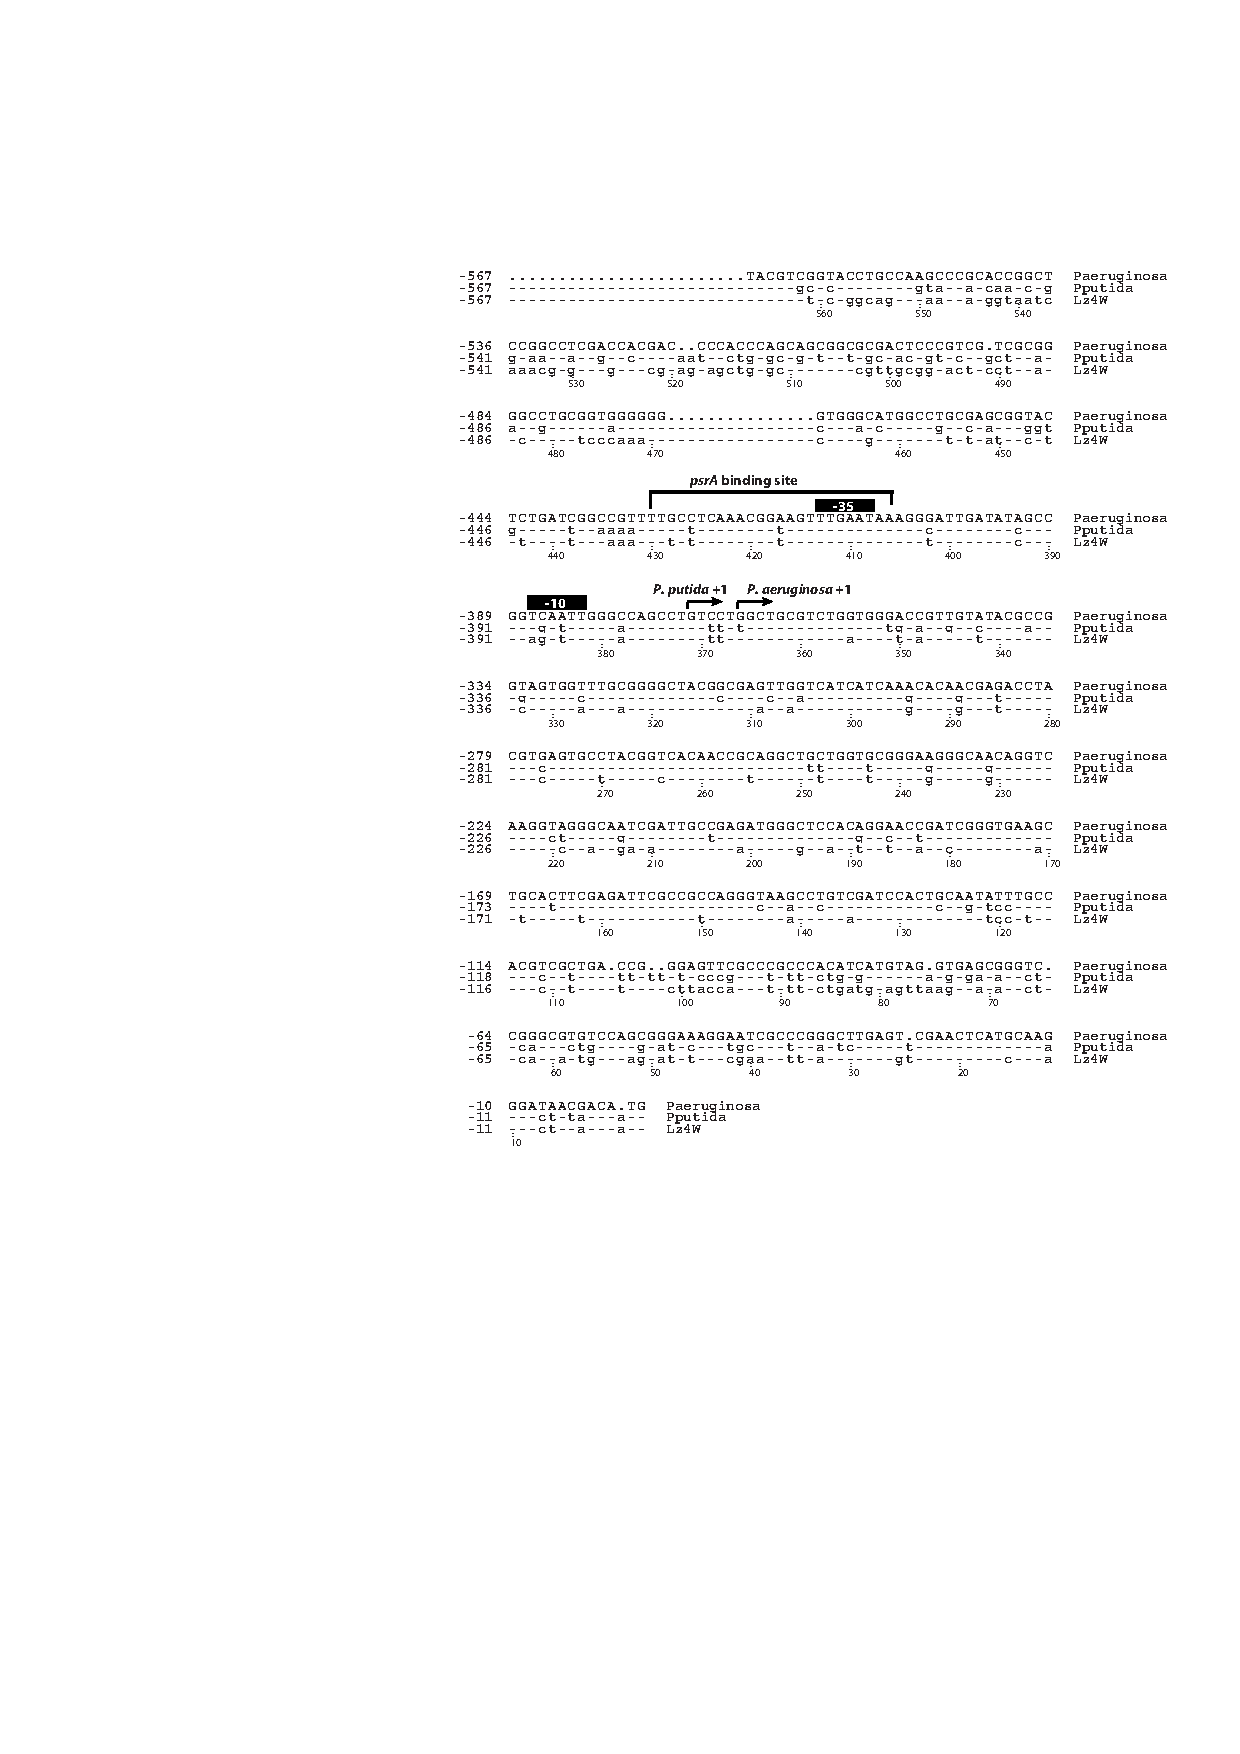
\includegraphics{figures/chap4_promoters}
\caption[Comparison of \e{rpoS} promoters]{Comparison of \e{rpoS}
promoters of Lz4W, \bact{Pa} (labelled as Paeruginosa), and \e{P.
putida} (labelled as Putida). The sequences are numbered
negatively in respect to translation initiation site. The
transcription start sites, $-$10, and $-$35 sites are indicated.
Gaps in the sequence are marked with dot and identical sequences
are marked with dash. The transcription start sites are taken from
\citet{Tanaka1994} for \bact{Pa} and \citet{Kojic2002} for \e{P.
putida}.} \label{chap4:promoters}
\end{figure}

\subsubsection{RNA secondary structure comparison}
\label{secondary} As discussed in Section~\ref{chap1:srna}, DsrA,
a small RNA (sRNA) in \bact{Ec}, binds to a stem-loop structure of
\e{rpoS} mRNA near the translation initiation region (TIR,
Figure~\ref{chap4:rna}A) and plays a major role in upregulation of
\sigs{} level at low
temperature~\citep{Lease2000,Lease2000b,Lease1998,Majdalani1998}.
A comparison of the secondary structures of TIRs of \e{rpoS} was
performed among \bact{Ec} and pseudomonad homologs
(Figure~\ref{chap4:rna}, to find out whether TIRs of pseudomonads
also form similar secondary structures.

\begin{sidewaysfigure}[tbp]
\centering
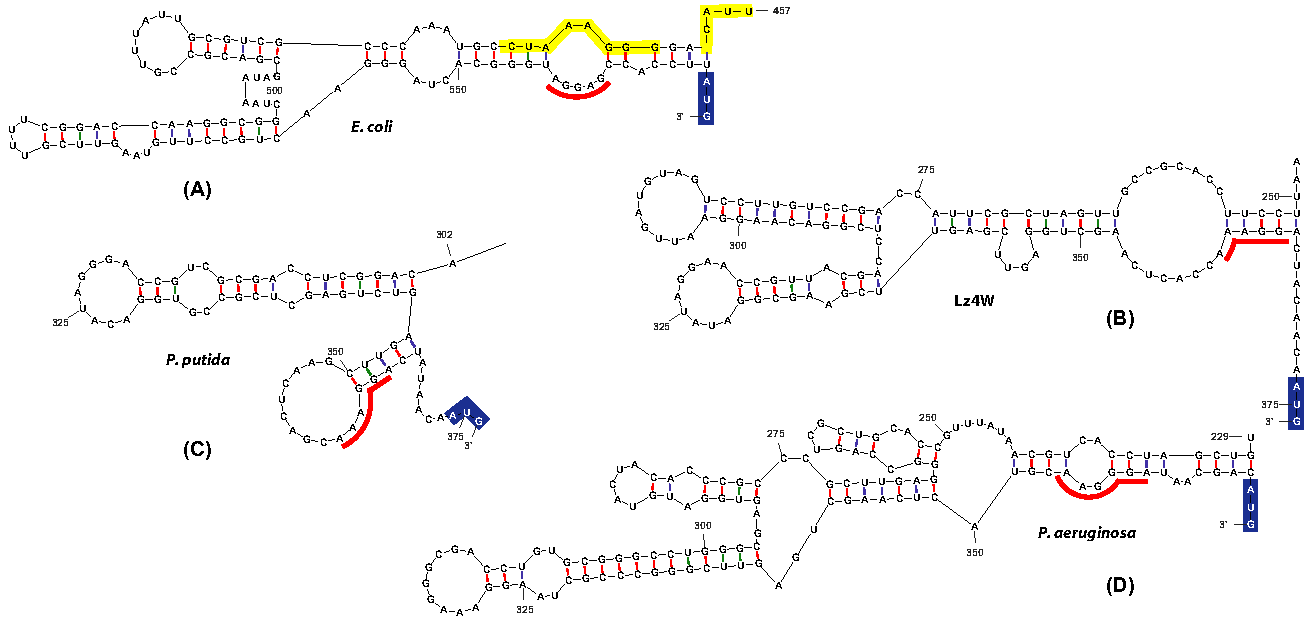
\includegraphics{figures/chap4_rna_structure}
\caption[RNA secondary structure comparison]{RNA secondary
structure comparison of the translation initiation regions of
\bact{Ec} \textbf{(A)}, Lz4W \textbf{(B)}, \e{P. putida}
\textbf{(C)}, and \bact{Pa} \textbf{(D)}\@. RNA sequence upstream
of the initiation codon (inclusive) to the transcription start
site were used for structure prediction by MFOLD version
3.1~\citep{Mathews1999}. Only the predicted lowest energy
structure of translation initiation region is shown in each case.
Putative ribosome binding sites are marked with red line,
initiation codon is colored blue, and the DsrA binding region in
\bact{Ec} structure is colored yellow. Note the numbering
increases towards the initiation codon.} \label{chap4:rna}
\end{sidewaysfigure}

The structures of the TIRs from \bact{Ec} and \bact{Pa}, although
very different in length (567 bases for \bact{Ec} and 366 bases
for \bact{Pa}), were strikingly similar. Both could potentially
form similar stem-loop structure involving ribosome binding site
(RBS), indicating both might be regulated by  similar mechanism. A
search in the genome sequence of \bact{Pa} with \bact{Ec} DsrA did
not find any significant hit. A search with the \bact{Pa}
stem-loop structure sequence ($-$229 to $-$242), however, returned
46 hits in the genome (data not shown). It remains to be seen
whether any of these hits are in fact DsrA homolog of \bact{Pa}.

TIRs of \e{P. putida} and Lz4W are, however, similar but different
from \bact{Ec} and \bact{Pa}. In first two instances, RBS is
almost completely buried within a stem (Figure~\ref{chap4:rna}B
and C), indicating a different regulation than that observed in
\bact{Ec} and \bact{Pa}.



\subsection{RpoS as phylogenetic tool}

Till date, outside of $\gammaup$ Proteobacteria, RpoS homologs
have been identified only in four species, three from $\betaup$
Proteobacteria and the other from \emph{Aquifex}. It is to be
noted that \emph{sigB} genes, in Gram positive bacteria, though
generally involved in stress response, are not homologs of RpoS.
From sequence alignnment, it is clear that all these three RpoS
sequences, obtained outside $\gammaup$ Proteobactaria are quite
diverged and can not be considered as RpoS homologs, unless
substantiated by biochemical and genetic data. It can therefore be
safely assumed that \emph{rpoS} gene is typically present only in
$\gammaup$ Proteobacteria.

\begin{figure}[tbp]
\begin{narrow}{-1.5in}{-1.5in}
\centering
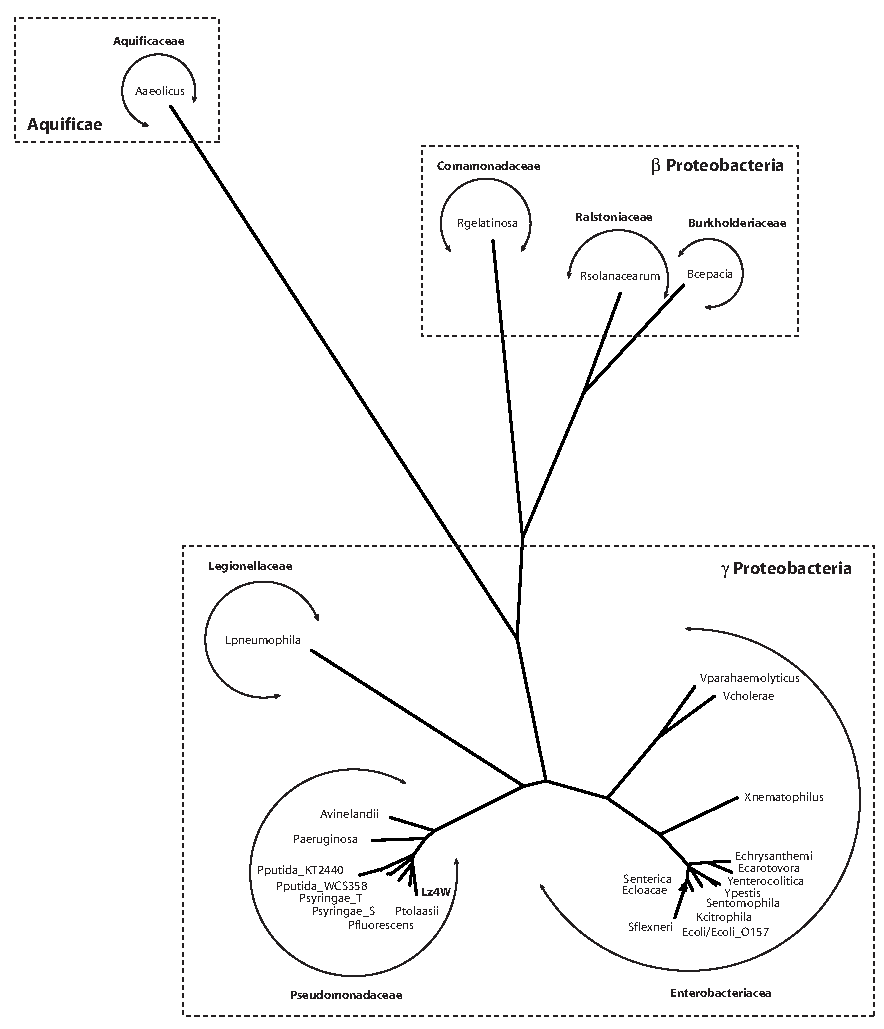
\includegraphics{figures/chap4_dendrogram}
\end{narrow}
\caption[Phylogenetic tree of RpoS sequences]{Fitch-Margoliash
tree for RpoS sequences available in SwissProt/TrEMBL. The tree
was generated by the method of \citet{Fitch1967} from the multiple
sequence alignment depicted in Figure~\ref{rpos_align}. The
distances were calculated using PROTDIST program of PHYLIP
package~\citep{Fel1989}.} \label{tree}

\end{figure}

A Fitch-Margoliash tree from the alignment distinctly supports
this conclusion (Figure~\ref{tree}). Moreover, the tree also shows
the clustering of the three groups within $\gammaup$
Proteobacteria. According to the tree, \bact{Pa} RpoS is different
from the rest of the pseudomonads. It is to be noted that the same
conclusion could be derived from the comparison of the TIR
secondary structure comparison (Section~\ref{secondary}). As shown
in Figure~\ref{tree}, the closest sequence to \Lzsigs{} is RpoS
sequence from \e{P. tolaasii}.


\section{Discussion}

In this Chapter the results of the sequence comparison of RpoD and
RpoS sequences, currently present in the sequence database, have
been presented. Sequence comparison of RpoD showed that the
fragment of \Lzsiga{}, which has been cloned in the present study,
is highly similar to its mesophilic counterpart, and identical in
several of its keys residue positions. Particularly important was
region 2.3, which has been shown to initiate the melting of the
DNA strand during open complex formation. \Lzsiga{} was identical
in these residues to other mesophilic RpoD sequences. Moreover,
RpoD sequences from several of the known cold-adapted bacteria did
not show any significant deviation from the mesophilic sequence.
This finding, therefore, indicates that the specific regulator of
promoter melting during transcription at low temperature, if any,
is not located in  region 2.3, but might lie in region 1.1 of the
\s{} factor, which was missing from the cloned fragment.

Sequence comparison and phylogenetic analysis of RpoS revealed
that the gene is largely present of $\gammaup$ Proteobacteria.
Several of the key residues in RpoS are very similar to the
residues of RpoD. The comparison also revealed that the amber
mutation within RpoS reading frame would result in a \s{} factor
lacking region 4.1 and 4.2. This is important from the viewpoint
of a recent finding~\citep{Campbell2002} that the \bact{Ec} RpoD
without regions 4.1 and 4.2 could transcribe from promoters with
\emph{extended} $-$10 motif. As would be seen in the later
Chapters of this thesis, the truncated form of \Lzsigs{} is also
functional, and could transcribe from \bact{Ec} promoters with
\emph{extended} $-$10 like motif.

Promoter comparison with the other pseudomonads identified the
putative $-$10 and $-$35 promoters elements of \lzsig{}. The
binding site for the TetR family member PsrA were conserved in all
the pseudomonads sequences examined, including \lzsig{}. The
comparison also revealed that the putative $-$10 element of
\lzsig{} deviates from the consensus sequence.

RNA secondary structure comparison revealed that the translation
initiation region (TIR) of \lzsig{} differs from \bact{Pa} and
\bact{Ec}. As the secondary structure at TIR is important for
\e{rpoS} regulation, the different structure would predict a
different regulation of \lzsig{} than that in \bact{Ec} and
\bact{Pa}. \ding{45}
